\documentclass[french,12pt,a4paper]{article}
\usepackage[T1]{fontenc}
\usepackage[utf8]{inputenc}
\usepackage[dvips]{graphicx}
%\usepackage[english]{babel}
\usepackage[frenchb]{babel}
\AddThinSpaceBeforeFootnotes % à insérer si on utilise \usepackage[french]{babel}
\FrenchFootnotes % à insérer si on utilise \usepackage[french]{babel}
\usepackage{amsmath,amsthm,amsfonts,amssymb}
\usepackage{mathrsfs}
\usepackage{array}
\usepackage{color}
\usepackage{float}
\usepackage{pstricks,pstricks-add,pst-plot,pst-tree}
\usepackage{enumerate}
\usepackage{textcomp}
\usepackage{lscape}
\usepackage{setspace}
\usepackage{lettrine}
\usepackage{lscape}
\usepackage{etex}
\usepackage{lmodern}
\usepackage{stmaryrd}
\usepackage{subfigure}
\usepackage{multido}
\usepackage{listings}
\usepackage{footnote}
\usepackage{appendix}
\usepackage{color}
\usepackage{listings}
\usepackage{tikz}
\usepackage{dsfont}
\usetikzlibrary{matrix}

\lstset{
  language={C++},
  numbers=left, numberstyle=\tiny, stepnumber=1, firstnumber=last,
  frameround=tttt, 
  frame=single, 
  float,
  captionpos=b,
  breaklines=true,
  sensitive=f,
  morestring=[d]",
  basicstyle=\small\ttfamily,
  keywordstyle=\bf\small,
  stringstyle=\sf
}
\usepackage{fancyhdr,lastpage}
\usepackage[twoside,left=2cm,top=2.5cm,dvips,marginparwidth=1.9cm,marginparsep=0.5cm,headheight=35pt]{geometry}
%En tete et pied de page
\usepackage{fancyhdr}
\pagestyle{fancy}
\lhead{\leftmark} 
\chead{}
\rhead{PEPS}
\lfoot{ENSIMAG 3A}
\cfoot{\textit{Equipe 7}}
\rfoot{\thepage}
\renewcommand{\headrulewidth}{0pt}  
\renewcommand{\footrulewidth}{0.4pt}
\title{Projet .NET : Gestion indicielle}
\date{October 31, 475}
\author{Guillaume Fuchs, Guillaume Pelletier, Louis Perfumo, Samuel Rosilio}
%Page de garde

\begin{document}
\begin{titlepage}
\begin{center}

\textsc{\LARGE ENSIMAG}\\[1.5cm]

\textsc{\Large Projet d'évaluation de produit structuré}\\[0.5cm]

% Title
 \hrule
 \hrule 

\vspace{7mm}
{ \huge \bfseries Playlist 2\\ Partie fonctionnelle  }

\vspace{7mm}
\hrule
\hrule

\vspace{7mm}
% Author and supervisor
\begin{minipage}{0.4\textwidth}
\begin{flushleft} \large
\emph{Etudiants:}\\
Guillaume \textsc{Fuchs},\\
Guillaume \textsc{Pelletier},\\
Samuel \textsc{Rosilio},\\
Louis \textsc{Perfumo}
\end{flushleft}
\end{minipage}

\vfill

% Bottom of the page
{\large \today}

\end{center}
\end{titlepage}
\tableofcontents
\newpage

\section{Moteur de calcul C++}
Le but de cette partie est d'expliquer la structure de l'outil permettant de calculer le prix de \textbf{Playlist 2}, le delta ainsi que le portefeuille de couverture par différente méthode de calcul et de simulation.\\
La section 1.1 présente le problème auquel on s'intéresse et les motivations pratiques. La section 1.2 présente l'architecture du moteur de calcul de notre outil. La section 1.3 explique dans le cadre du modèle de Black Scholes les différents algorithmes utilisés pour le calcul du prix, du delta et de la couverture.

\subsection{Motivations pratiques}
Durant l'ensemble de la description  des algorithmes utilisés dans notre outils nous noterons $S = (S_{t}, t \geq 0)$ la dynamique du sous-jacent et $\mathcal{F}$ sa filtration naturelle. Pour simplifier les choses, nous allons supposer que le payoff du produit s'écrit sous la forme:
$$\phi(S_{t_{0}},...,S_{t_{N}}) $$
où $0 = t_{0} \leq ... \leq t_{N} = T$ est une grille de dates de constatations non-forcément équi-réparties.\\\\
Notons $r$ le taux d'intérêt instantané que nous supposerons pour l'instant constant. Le prix à l'instant $0 \leq t \leq T$, avec $t_{i} \leq t \leq t_{i+1}$ du produit est donné par:
$$\upsilon(t, S_{t_{0}},...,S_{t_{N}}) = e^{-r(T-t)}\mathbb{E}(\phi(S_{t_{0}},...,S_{t_{N}})\mid\mathcal{F})$$

\subsection{Architecture}
% Image de l'architecture + commentaires

\begin{center}
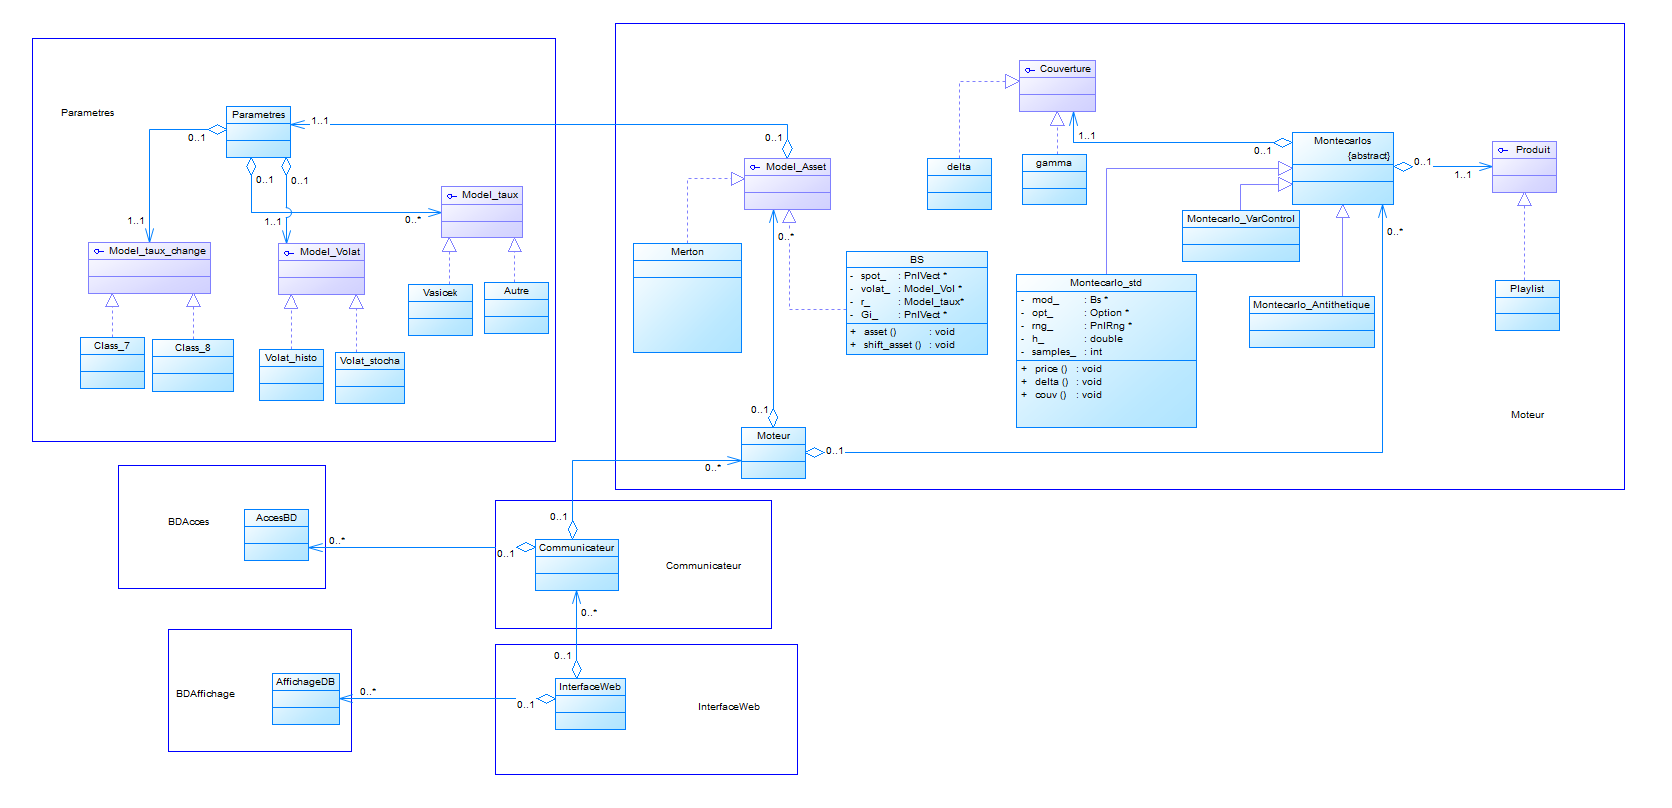
\includegraphics[scale=0.3]{Img/Architecture.png}
\end{center}


\subsection{Modèle de Black-Scholes}
Considérons $D$ indices évoluant chacun selon le modèle de Black Scholes et corrélés entre eux. La dynamique $S$ de ces $D$ indices s'écrit:
$$ S_{t}^{d} = S_{0}^{d}e^{(r-\frac{(\sigma^{d})^{2}}{2})t+\sigma^{d}B_{t}^{d}}, \hspace{7 mm} d=1,...D$$
où $r$ est le taux d’intérêt, $(\sigma^{1},..., \sigma^	{d})$ sont les volatilités de chacun des indices que nous supposerons constant et $B = (B^{1},...,B^{D})^{T}$ est un vecteur de $D$ mouvements Browniens standards et réels de matrice de corrélation $Cov(B_{t},B_{t}) = \Gamma t$ définie par $Cov(B^{i}_{t} ,B^{j}_{t} ) = \Gamma_{ij}t$ avec $\Gamma_{ij} = \rho$ pour tout $i \neq j$ et $\Gamma_{ii} = 1$. Le paramètre $\rho$ doit être choisi dans $] -\frac{1}{D-1} , 1[$ de telle sorte que $\Gamma$ soit définie positive pour assurer que le marché soit complet. Attention $B$ n’est pas un mouvement Brownien standard à valeurs dans $\mathbb{R}^{D}$ car ses composantes ne sont pas indépendantes mais on peut le réécrire en utilisant un mouvement Brownien standard à valeurs dans $\mathbb{R}^{D}$, noté dans la suite $W = (W^{1}, . . . ,W^{d})^{T}$ et qui sera vu comme un vecteur colonne. Ainsi on a l’égalité en loi $(B_{t}, t \geq 0) = (LW_{t}, t \geq 0)$ pour tout $t \geq 0$ où $L$ est la factorisée de Cholesky de la matrice $\Gamma$, .i.e $\Gamma = L'L$ avec $L$ triangulaire inférieure. L’équation de la dynamique se réécrit alors:
$$ S_{t}^{d} = S_{0}^{d}e^{(r-\frac{(\sigma^{d})^{2}}{2})t+\sigma^{d}L^{d}W_{t}}, \hspace{7 mm} d=1,...D $$
où $L^{d}$ est la ligne $d$ de la matrice $L$. Ainsi la quantité $L^{d}W_{t}$ est bien un réel. De cette équation, on remarque facilement que l’on peut déduire:
$$ S_{t}^{d} = S_{0}^{d}e^{(r-\frac{(\sigma^{d})^{2}}{2})t+\sigma^{d}L^{d}(W_{t_{i+1}}-W_{t_{i}})}, \hspace{7 mm} d=1,...D $$
$$ S_{t}^{d} = S_{0}^{d}e^{(r-\frac{(\sigma^{d})^{2}}{2})t+\sigma^{d}\sqrt{(t_{i+1}-t_{i})}L^{d}G_{i+1}}, \hspace{7 mm} d=1,...D $$

où la suite $(G_{i})_{i \geq 1}$ une suite i.i.d de vecteurs gaussiens centrés de matrice de covariance identité. Ainsi pour simuler le processus $S$ sur la grille $(t_{i})_{i=0,...,N}$ il suffit de savoir simuler des vecteurs gaussiens centrés de matrice de covariance identité.\\

\subsubsection{Prix}
\textbf{Prix à l'instant 0}\\
Le prix à l'instant 0 est donné
$$ \upsilon(0, S_{0}) = e^{-rT}\mathbb{E}(\phi(S_{t_{0}},...,S_{t_{N}})$$
On approche $\upsilon(0, S_{0})$, grâce à une méthode de Monte Carlo, par
$$ e^{-rT}\frac{1}{M}\sum_{j=1}^{M} \phi(S_{t_{0}}^{(j)},...,S_{t_{N}}^{(j)})$$
où les $N$-uplets $(S_{t_{0}}^{(j)},...,S_{t_{N}}^{(j)})$ pour $j=1,...,M$ sont i.i.d selon la loi de $(S_{t_{0}},...,S_{t_{N}})$.\\

\textbf{Prix à l'instant $t>0$}\\
Pour calculer le prix à l'instant $t$, il faut calculer une espérence conditionnelle. Lorsque cela est possible, une manière de traiter le calcul de cette espérence conditionnelle est de réécrire le sous-jacent $S_{t+u}$ à l'instant $t+u$ pour $u>0$ en fonction de la valeur $S_{t}$ d’un sous–jacent à l’instant $t$ et d’une quantité indépendante de $\mathcal{F}_{t}$:
$$ S_{t+u} = S_{t}e^{(r-\frac{\sigma^{2}}{2})u+\sigma(B_{t+u}-B_{t})} = S_{t}\tilde{S_{u}}$$
où $\tilde{S_{u}}$ est \textbf{indépendant} de $\mathcal{F}_{t}$ ie indépendant du passé jusqu'à $t$ inclus et la dynamique de $\tilde{S}$ est donnée par
$$ \tilde{S_{u}} = e^{(r-\frac{\sigma^{2}}{2})u+\sigma\tilde{B_{u}}}$$
où $\tilde{B}$ est un mouvement Brownien réel standard indépendant de $\mathcal{F_{t}}$. On a donc:
$$ S_{t_{i+1}} \stackrel{Loi}{=} S_{t_{i}}e^{(r-\frac{\sigma^{2}}{2})(t_{i+1}-t_{i})+\sigma\sqrt{t_{i+1}-t_{i}}G_{i+1}} $$
où $(G_{i+1})_{i\geq0}$ est une suite i.i.d selon la loi normale centrée réduite.

Ainsi le prix à l’instant t se réécrit
$$\upsilon(t, S_{t_{0}},..., S_{t_{i}},S_{t}) = e^{-r(T-t)}\mathbb{E}((\phi(s_{t_{0}},...,s_{t_{i}},S_{t_{i+1}},...,S_{t_{N}}))$$

Les lettres s minuscules désignent des variables déterministes. On peut alors approcher le prix
à l’instant t par la moyenne Monte Carlo suivante:
$$ e^{-r(T-t)}\frac{1}{M}\sum_{j=1}^{M} \phi(s_{t_{0}},...,s_{t_{i}},S_{t_{i+1}}^{(j)}...,S_{t_{N}}^{(j)})$$
Les quantités $(s_{t_{0}},s_{t_{1}},...,s_{t_{i}},s_{t})$ représentent les valeurs réellement observées jusqu’à l’instant $t$ sur la trajectoire du sous-jacent sur laquelle on souhaite calculer le prix du produit. D’un point du vue pratique, les valeurs $(s_{t_{0}},s_{t_{1}},...,s_{t_{i}},s_{t})$ sont les cotations du sous-jacent observées sur le marché jusqu’à la date $t$.

\subsubsection{Delta}

Pour construire notre portefeuille de couverture, nous appliquerons une \textit{couverture en delta}. Ce portefeuille est entièrement déterminé par la quantité d'actifs risqués à posséder à chaque instant $t$ qui est donnée par la dérivée du prix par rapport à $S_{t}$, ie
$$ \frac{\delta\upsilon(t, S_{t_{0}},.., S_{t_{i}}, S_{t})}{\delta S_{t}} $$
Cette quantité est connue sous le nom de delta du produit et sera approché par une méthode de différence finies associé à une méthode de Monte Carlo:
$$ \frac{e^{-r(T-t)}}{M2s_{t}h}\sum_{j=1}^{M}(\phi(s_{t_{0}},...,s_{t_{i}},(1+h)S_{t_{i+1}},...,(1+h)S_{t_{N}})-\phi(s_{t_{0}},...,s_{t_{i}},(1-h)S_{t_{i+1}},...,(1-h)S_{t_{N}}))$$
Pour un produit faisant intervenir $D$ sous-jacents (4 dans notre cas), son portefeuille de couverture contient les $D$ actifs et la quantité d'actifs $d$ à détenir à l'instant $t$ est donnée par:
$$ \frac{\delta\upsilon(t, S_{t_{0}}^{d},...,S_{t_{i}}^{d},S_{t}^{d})}{\delta S_{t}^{d}} $$

\subsubsection{Couverture}

La répartition du \textit{P\&L} (Profit and Loss, ie erreur de couverture) joue un rôle central. Un modèle est jugé sur sa bonne capacité à couvrir les produits exotiques.\\
Considérons un actif dont la valeur du sous-jacent est noté $S_{t}$. Son évolution se fait sur une grille de temps {$t_{0}$,...,$t_{N}$} de pas $T/N$ où ${t_{0}}$ = $0$, le début de l'option et ${t_{N}}$ = $T$, la maturité de l'option sur le sous-jacent.\\
La méthode \lstinline!simul_market! de la classe \lstinline!BS! renvoi une simulation du marché avec un nombre de dates $H$. On considère la grille de discrétisation de pas $\frac{T}{H}$ avec
$$(\tau_{0},...,\tau_{N}) \supset (t_{0},...,t_{N})$$ 
où
 $\tau_{0}$ = $0$ et $\tau_{N}$ = $T$.\\
Le long de cette trajectoire, la construction du portefeuille de couverture se fait par le calcul du prix $p_{i}$ et du delta $\delta_{i}$ à chaque date $\tau_{i}$. L'évolution de la part investie au taux sans risque s'écrit:\\
$$
  \left\{%
     \vspace{-3ex}
        \begin{aligned}
          & V_{0} = p_{0}-\delta_{0}.S_{0} \\
          & V_{i} = V_{i-1}*\exp^{\frac{r*T}{H}}-(\delta_{i}-\delta_{i-1}).S_{\tau_{i}}, \hspace{7 mm}  i=1,...,H 
        \end{aligned}
 \right.
 $$
\\
L'erreur de couverture est donnée par:
 $$P\&L = V_{H}+\delta_{H}.S_{\tau_{H}}-payoff$$
\end{document}

